% Intended placement: Section 3.5, after member 2's AdaIN method.
\subsection{Structure-Preserving Style Augmentation}
\label{sec:structure_preserving}

We reuse member 2's frozen AdaIN encoder and decoder~\cite{huang2017adain} and
independently implement the structure map, spatial strength rule, and offline
generation pipeline. The content image $I_c$ is drawn only from Photo Training.
Its style image $I_s$ is read from the same frozen external pool and content--style
pairing used by ordinary AdaIN.

\textit{Structure map.} After resizing the shorter content side to 512 pixels,
we form grayscale intensity $Y=0.299R+0.587G+0.114B$ and smooth it with a Gaussian
kernel of standard deviation 1, giving $J=G_1*Y$. Let $K_x$ and $K_y$ be the
$3\times3$ Sobel kernels, scaled by $1/8$. The gradient response is
\begin{equation}
g=\sqrt{(K_x*J)^2+(K_y*J)^2}.
\label{eq:m3_gradient}
\end{equation}
Responses at most $10^{-6}$ are treated as zero. We set $s$ to the 95th percentile
of $g$; if that value is at most $10^{-6}$, we use the maximum response instead.
With $\epsilon=10^{-6}$, the soft structure map is
\begin{align}
\hat g&=\operatorname{clip}_{[0,1]}\!\left(\frac{g}{\max(s,\epsilon)}\right),\notag\\
M&=\operatorname{clip}_{[0,1]}\!\left(G_2*\operatorname{MaxPool}_{3\times3}(\hat g)\right).
\label{eq:m3_structure}
\end{align}
Maximum pooling uses stride 1 and preserves image size. It broadens thin responses;
the second Gaussian, with standard deviation 2, softens their transition.
Constant images receive a zero map. Generation uses this continuous response,
rather than a Canny mask or a learned saliency model.

\textit{Adaptive strength and feature mixing.} For base style strength $\alpha_0$
and protection parameter $\beta$, we define
\begin{equation}
\alpha(x,y)=\alpha_0[1-\beta M(x,y)],
\qquad \alpha_0,\beta\in[0,1].
\label{eq:m3_alpha}
\end{equation}
The map is area-averaged to the content encoder's \texttt{relu4\_1} resolution,
giving $\alpha_f$. Let $F_c=E(I_c)$ and $F_s=E(I_s)$. The decoder input and output are
\begin{align}
F_{\mathrm{mix}}&=\alpha_f\odot\operatorname{AdaIN}(F_c,F_s)\notag\\
               &\quad +(1-\alpha_f)\odot F_c,\label{eq:m3_mix}\\
I_{\mathrm{sp}}&=D(F_{\mathrm{mix}}).\label{eq:m3_decode}
\end{align}
The one-channel map broadcasts over the 512 feature channels. Strong structure
responses reduce the style contribution. At $\beta=0$, the rule reduces to
ordinary constant-strength AdaIN; this equivalence is verified in the implementation.
At $\alpha_0=0$, the result is an encoder--decoder reconstruction, not an exact
copy of the input. Figure~\ref{fig:m3_maps} visualizes the actual maps; the complete
pipeline is shown in Fig.~\ref{fig:m3_pipeline}.

\begin{figure}[t]
\centering
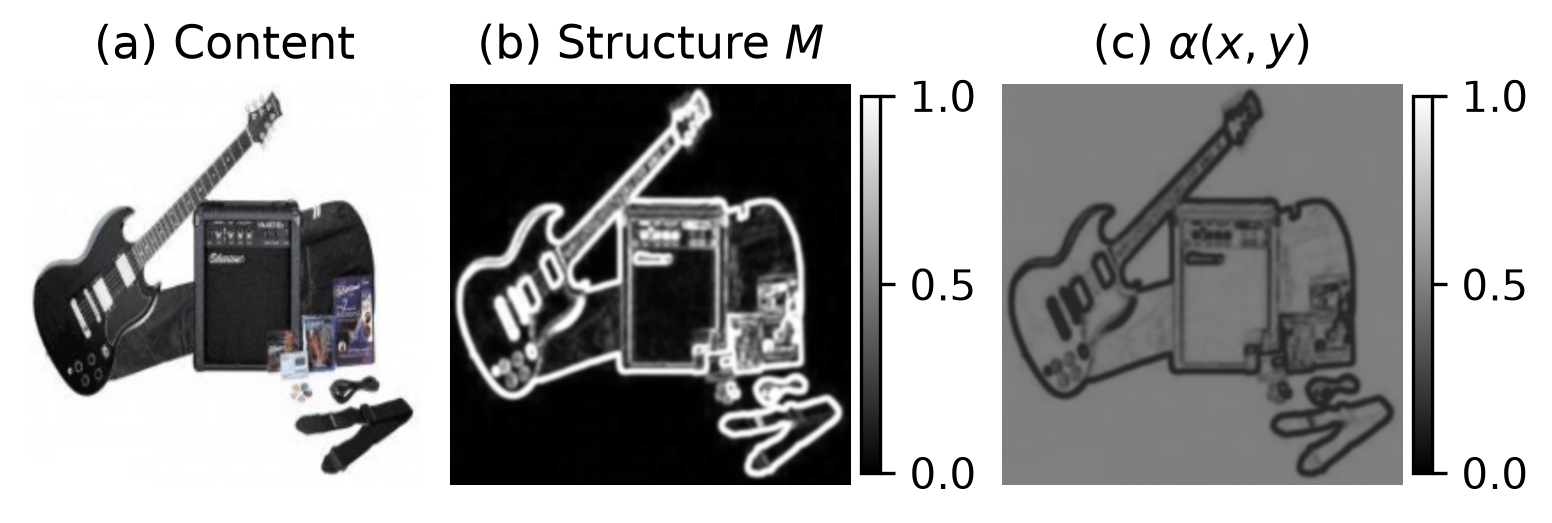
\includegraphics[width=\columnwidth]{m3_structure_alpha.png}
\caption{Actual Photo Training example: content image, soft structure response
$M$, and spatial strength $\alpha(x,y)$ for $\alpha_0=0.5$, $\beta=0.7$.
Both map color scales are fixed to $[0,1]$. Brighter $M$ produces lower local
style strength. The map also responds to background contours.}
\label{fig:m3_maps}
\end{figure}

\begin{figure*}[t]
\centering
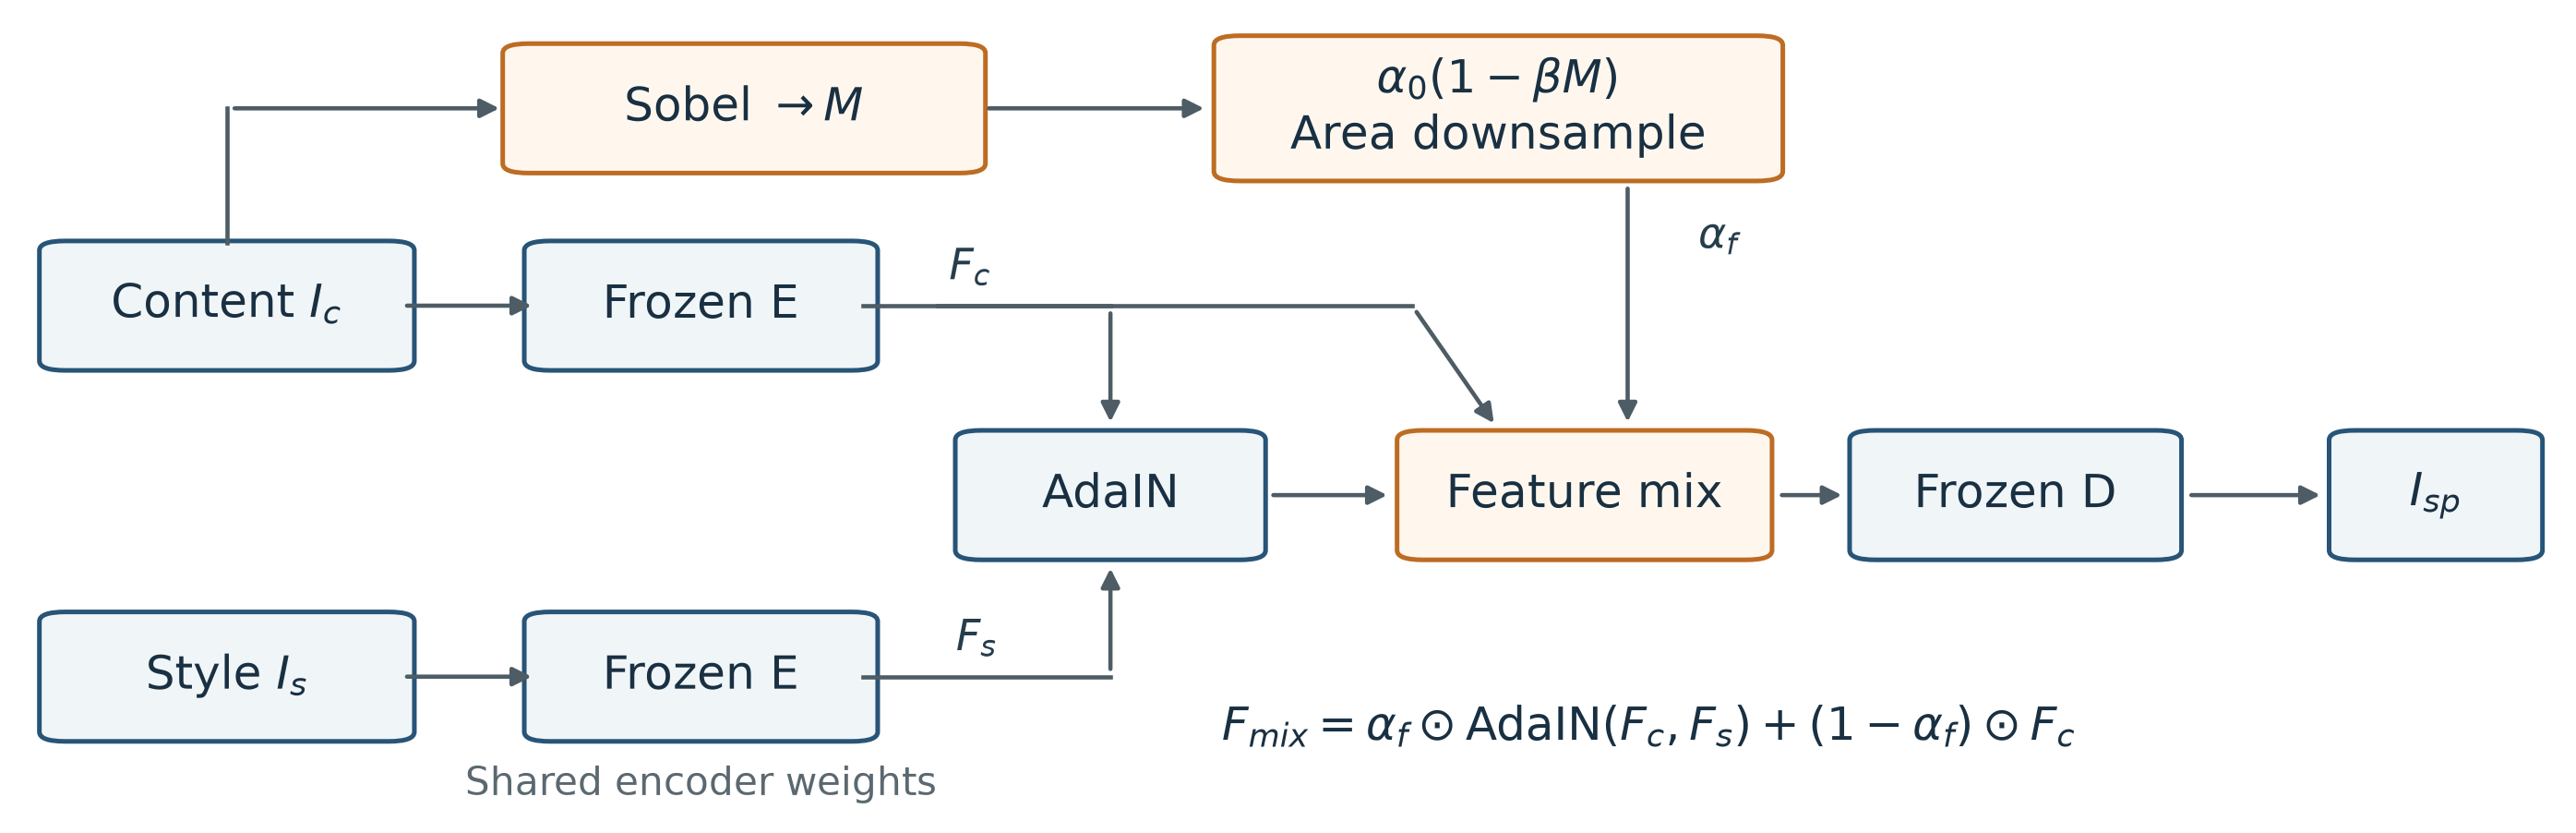
\includegraphics[width=0.96\textwidth]{m3_pipeline.png}
\caption{Structure-guided feature mixing. The structure branch uses the content
image only; the style reference changes feature statistics. Encoder and decoder
weights remain frozen.}
\label{fig:m3_pipeline}
\end{figure*}

\textit{Offline delivery and limitations.} The initial full set uses
$\alpha_0=0.5$, $\beta=0.7$ and contains one output for each of the 1,349 source
training images. The latter parameter is an initial setting, not a selected optimum.
Images are written to \texttt{data/aug\_sp/}; a manifest records the output path,
label, original, style, $\alpha_0$, and $\beta$. Geometry, frozen weights,
content--style pairing, and JPEG quality 95 are held fixed relative to the matched
AdaIN reference. Output dimensions follow the same decoder behavior in both
methods. The map is an edge-based proxy and cannot guarantee object preservation
after decoding. Since the rule also lowers mean style strength, a uniform control
with matched mean strength is needed to isolate the effect of spatial placement.
